\subsection{Input Features for QoE Prediction}
\label{BiLSTM:subsec:InputFeatures}


\begin{figure}[tb]
  \centering
  \begin{subfigure}{0.48\linewidth}
    \centering
    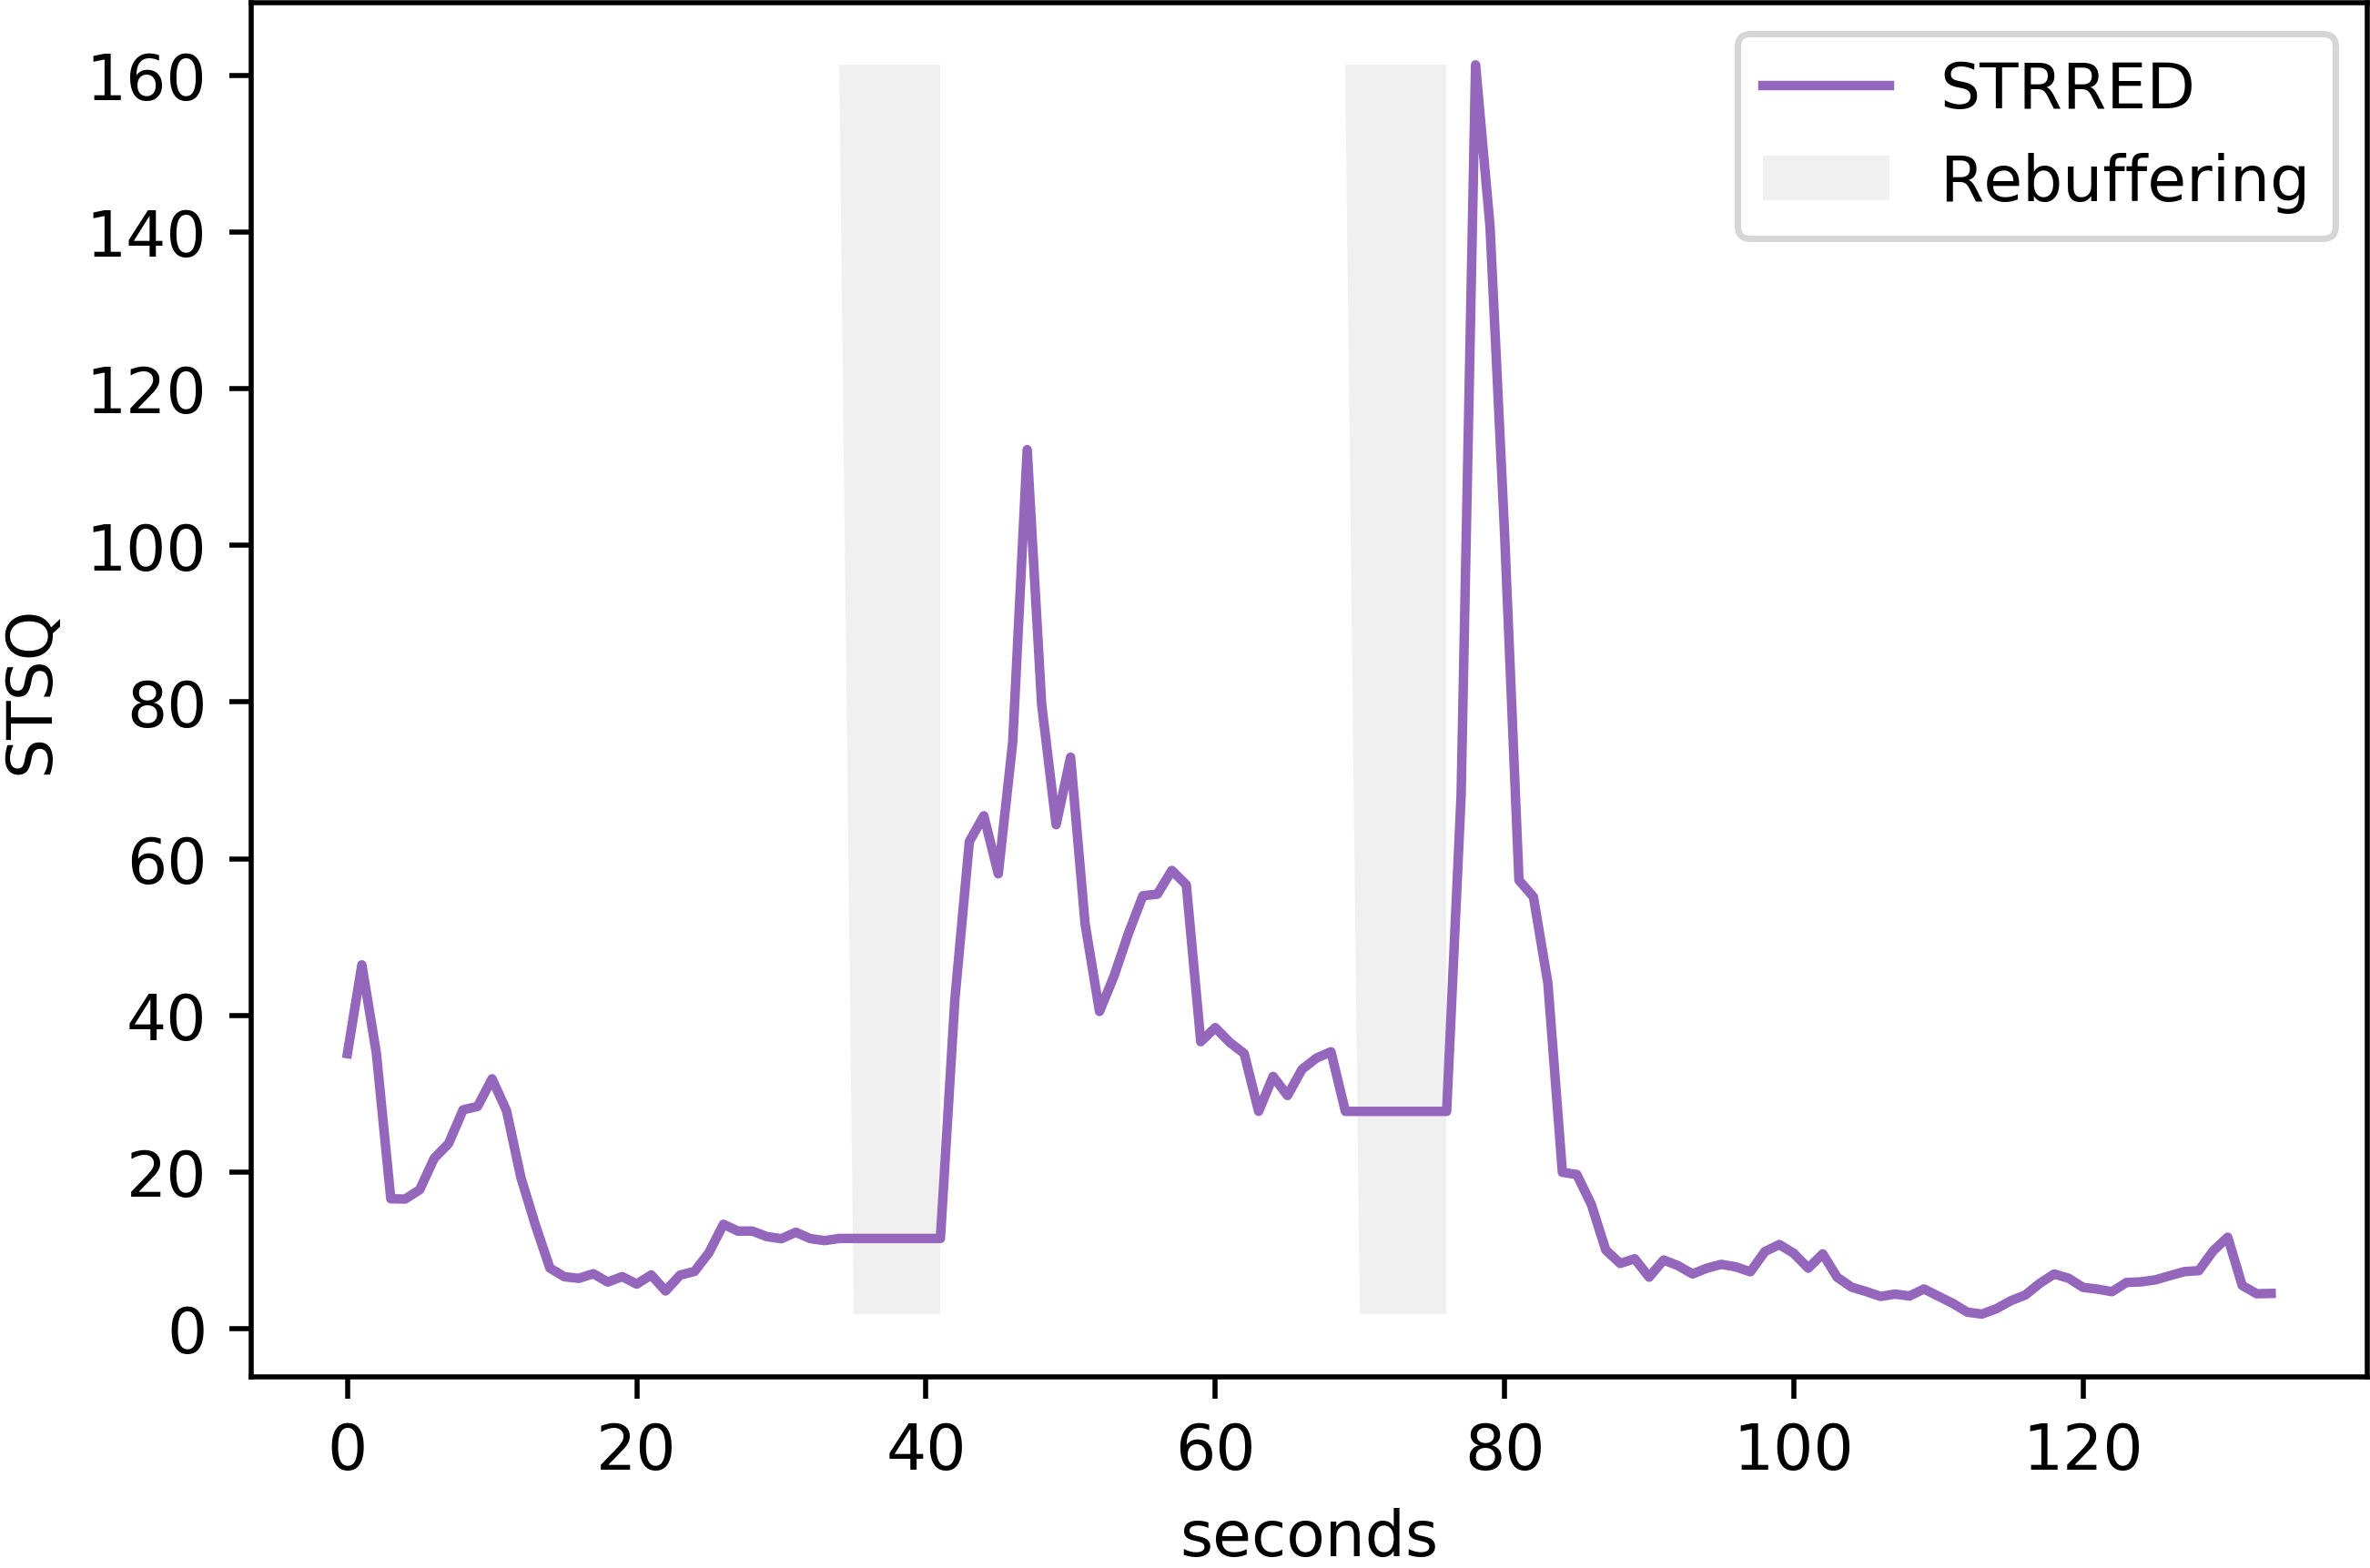
\includegraphics[width=\textwidth]{\FigsDir/features_STSQ.png}
    \caption{STSQ}
    \label{fig:InputFeatures_STSQ}
  \end{subfigure}
  \hfill
  \begin{subfigure}{0.48\linewidth}
    \centering
    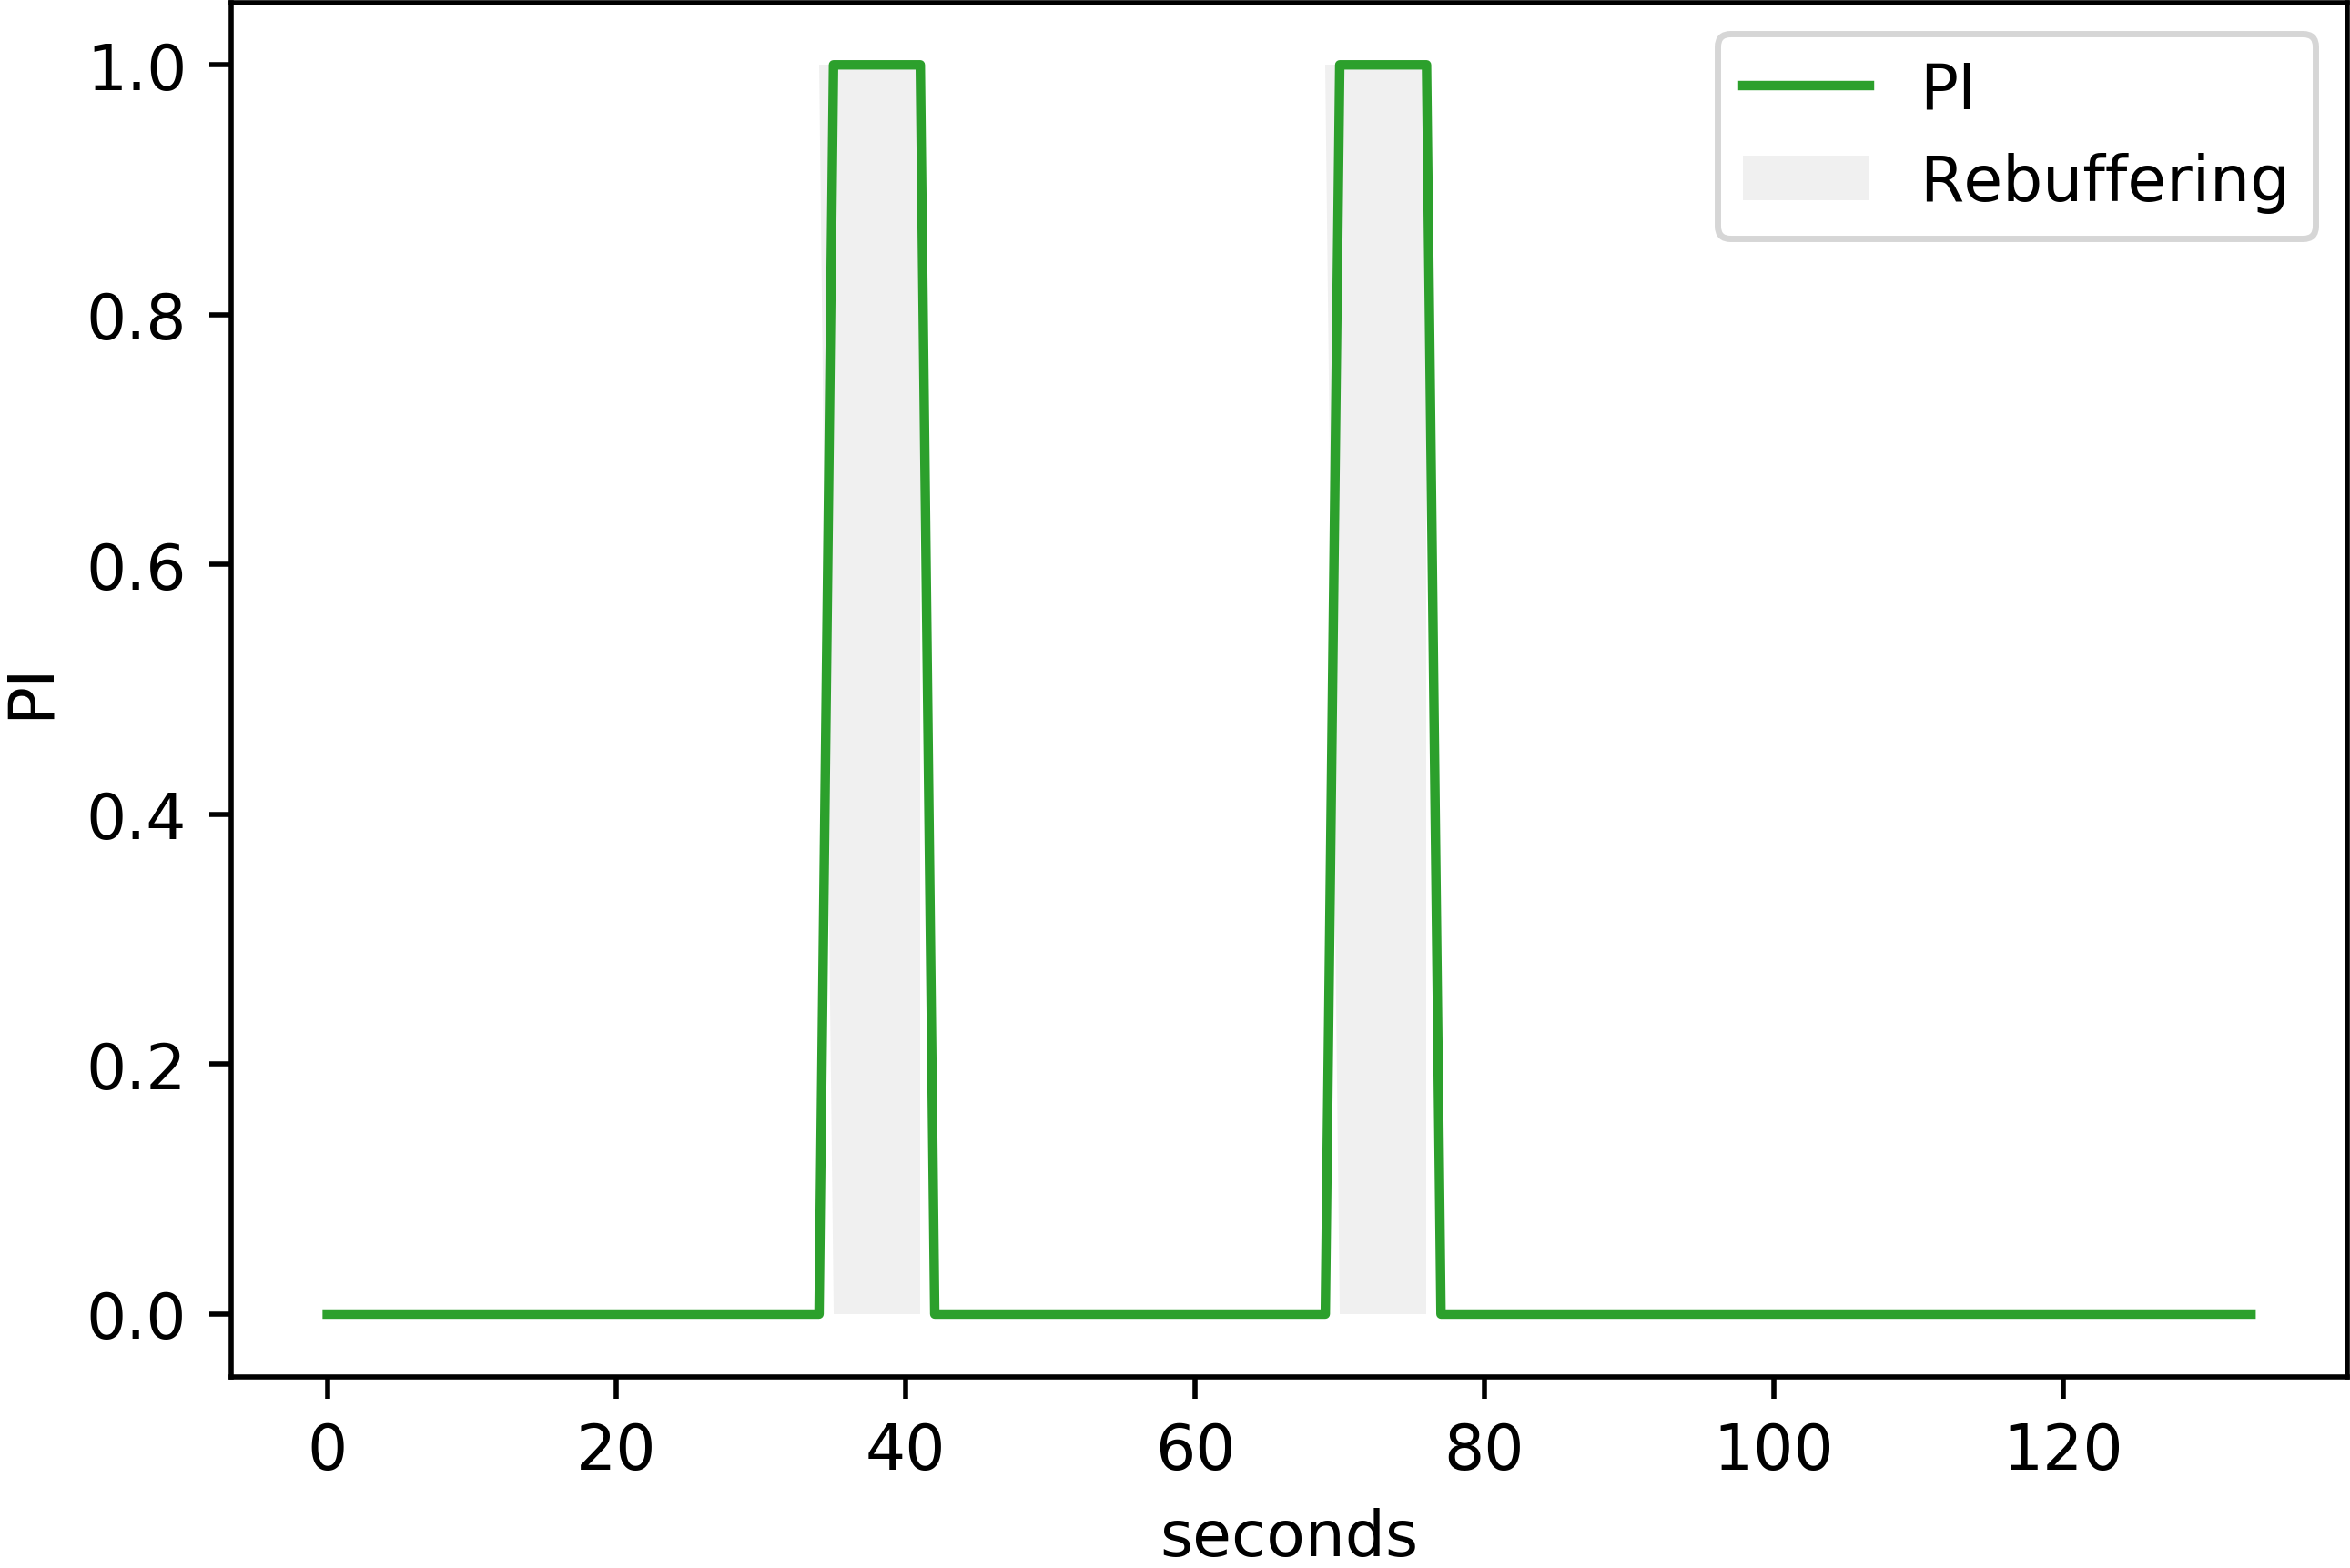
\includegraphics[width=\textwidth]{\FigsDir/features_PI.png}
    \caption{PI}
    \label{fig:InputFeatures_PI}
  \end{subfigure}
  
  \vspace{6pt}
  
  \begin{subfigure}{0.48\linewidth}
    \centering
    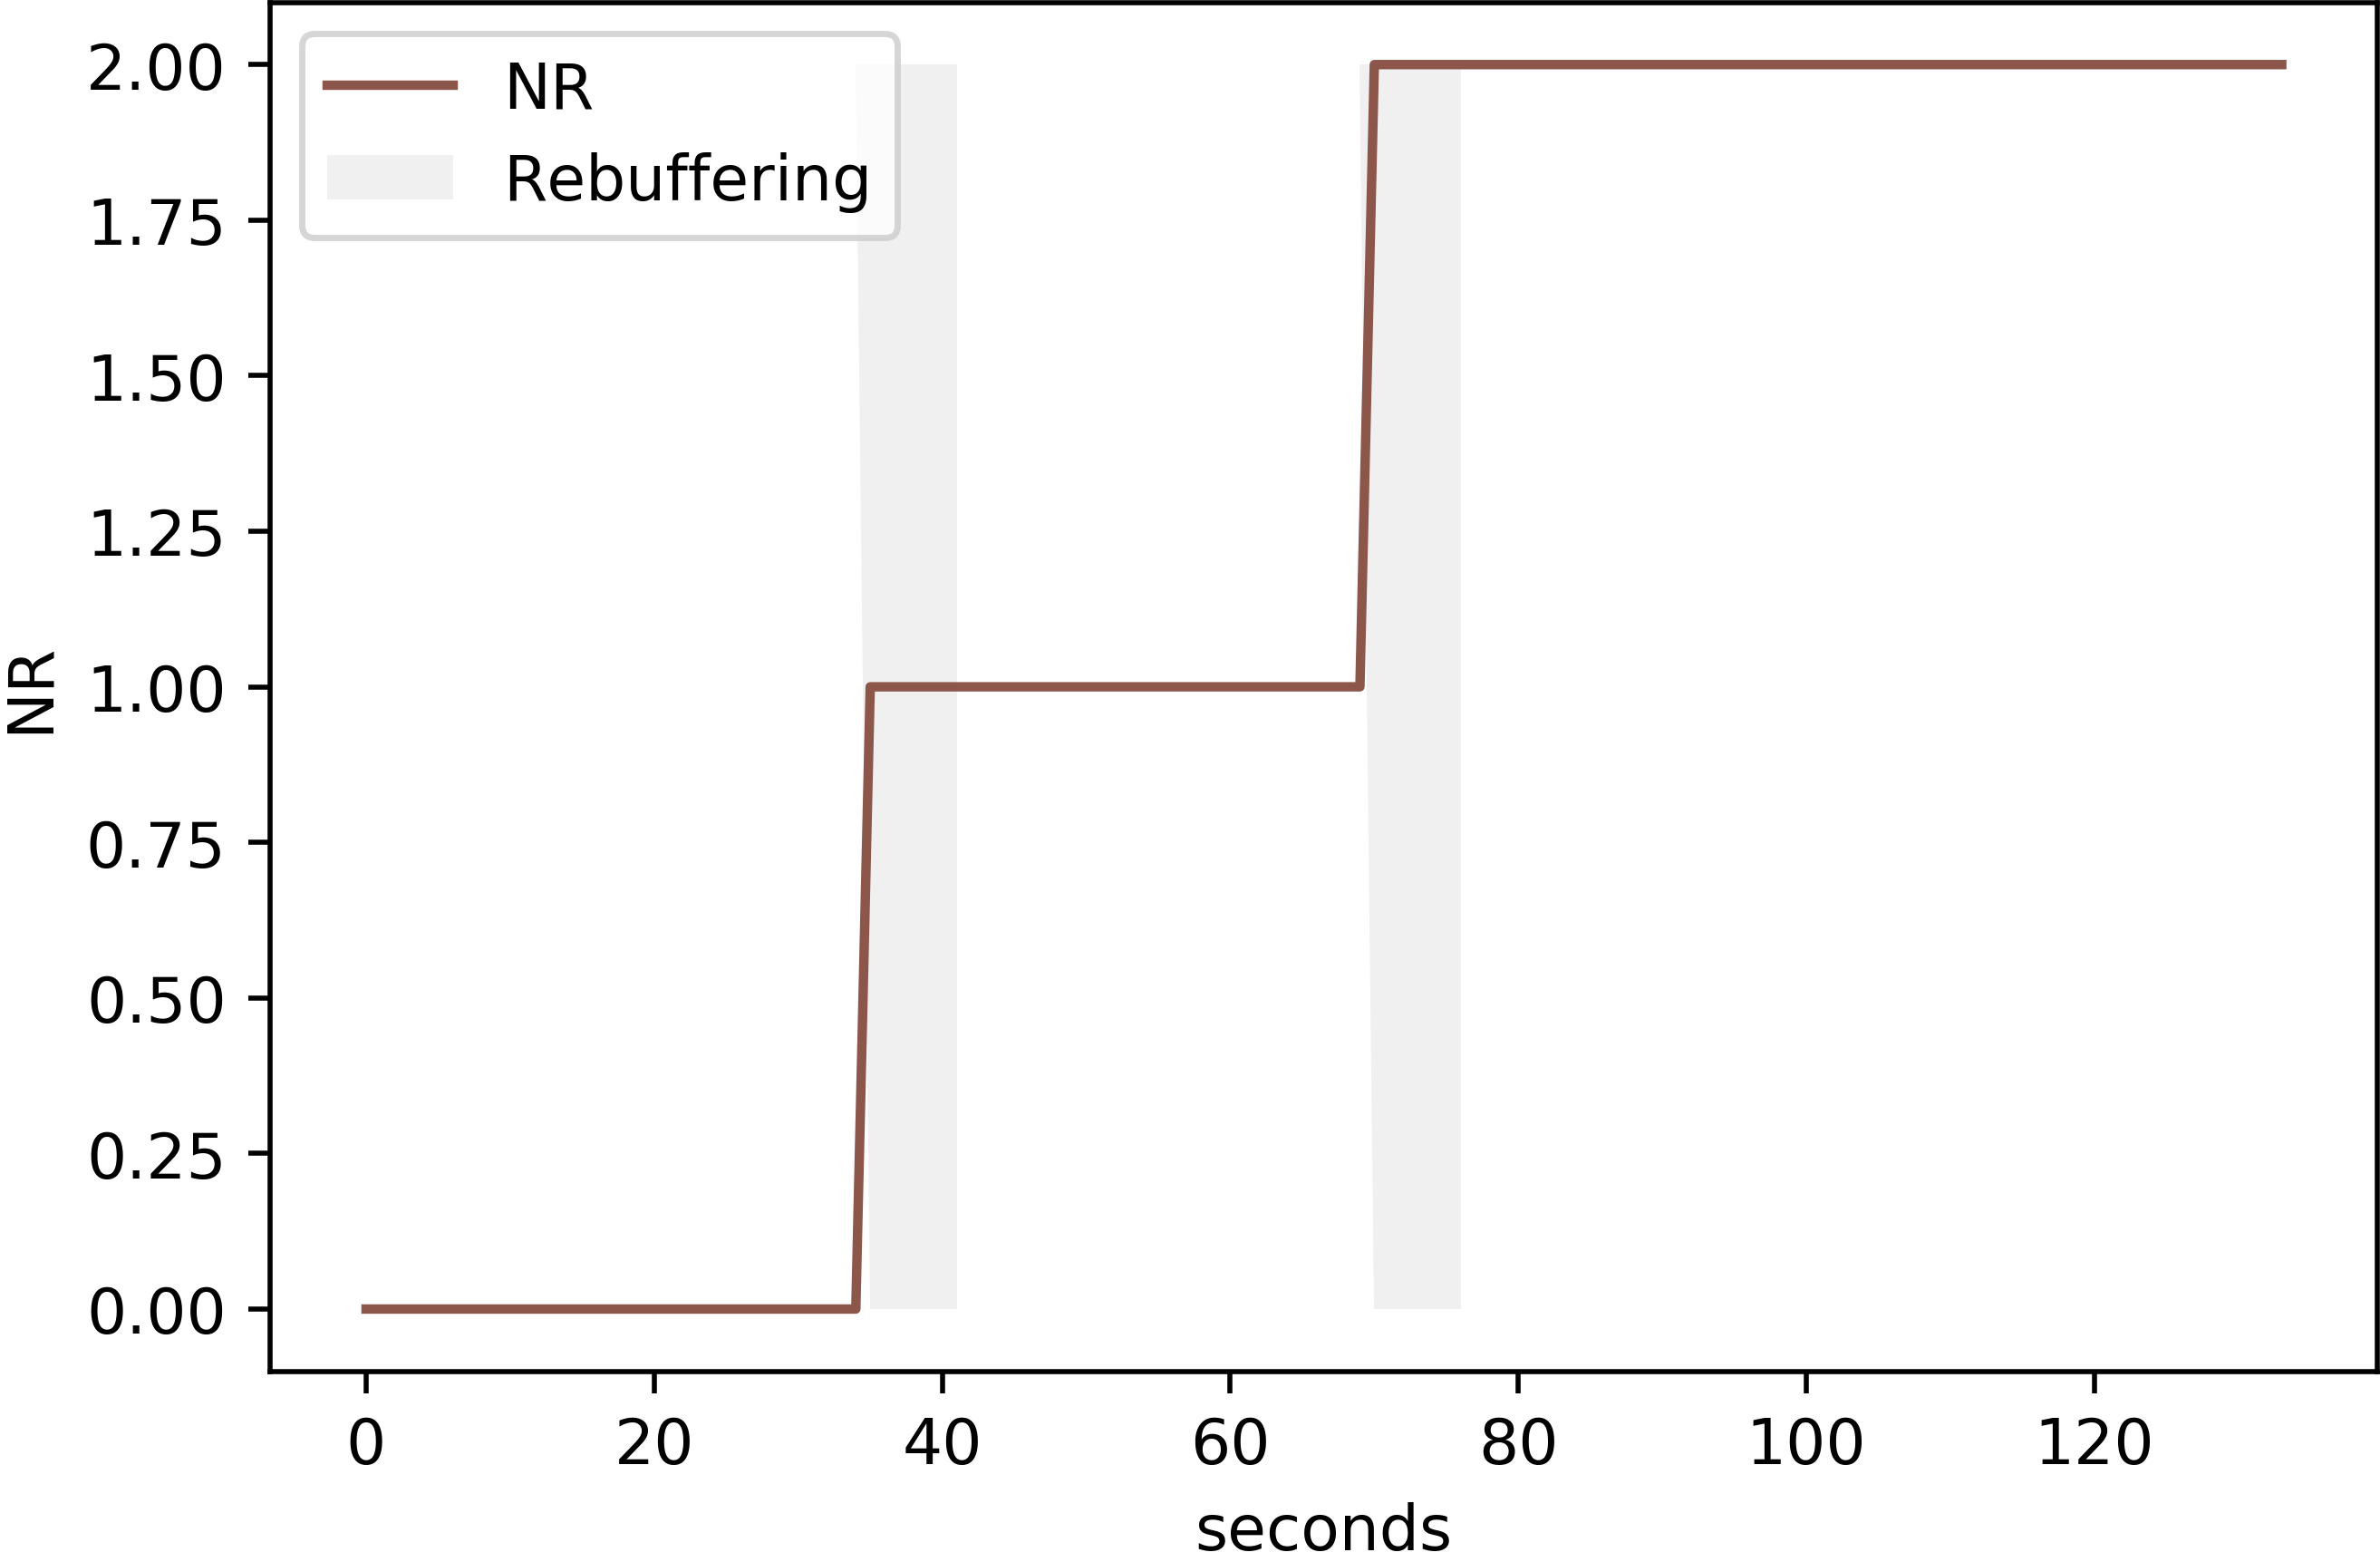
\includegraphics[width=\textwidth]{\FigsDir/features_NR.png}
    \caption{NR}
    \label{fig:InputFeatures_NR}
  \end{subfigure}
  \hfill
  \begin{subfigure}{0.48\linewidth}
    \centering
    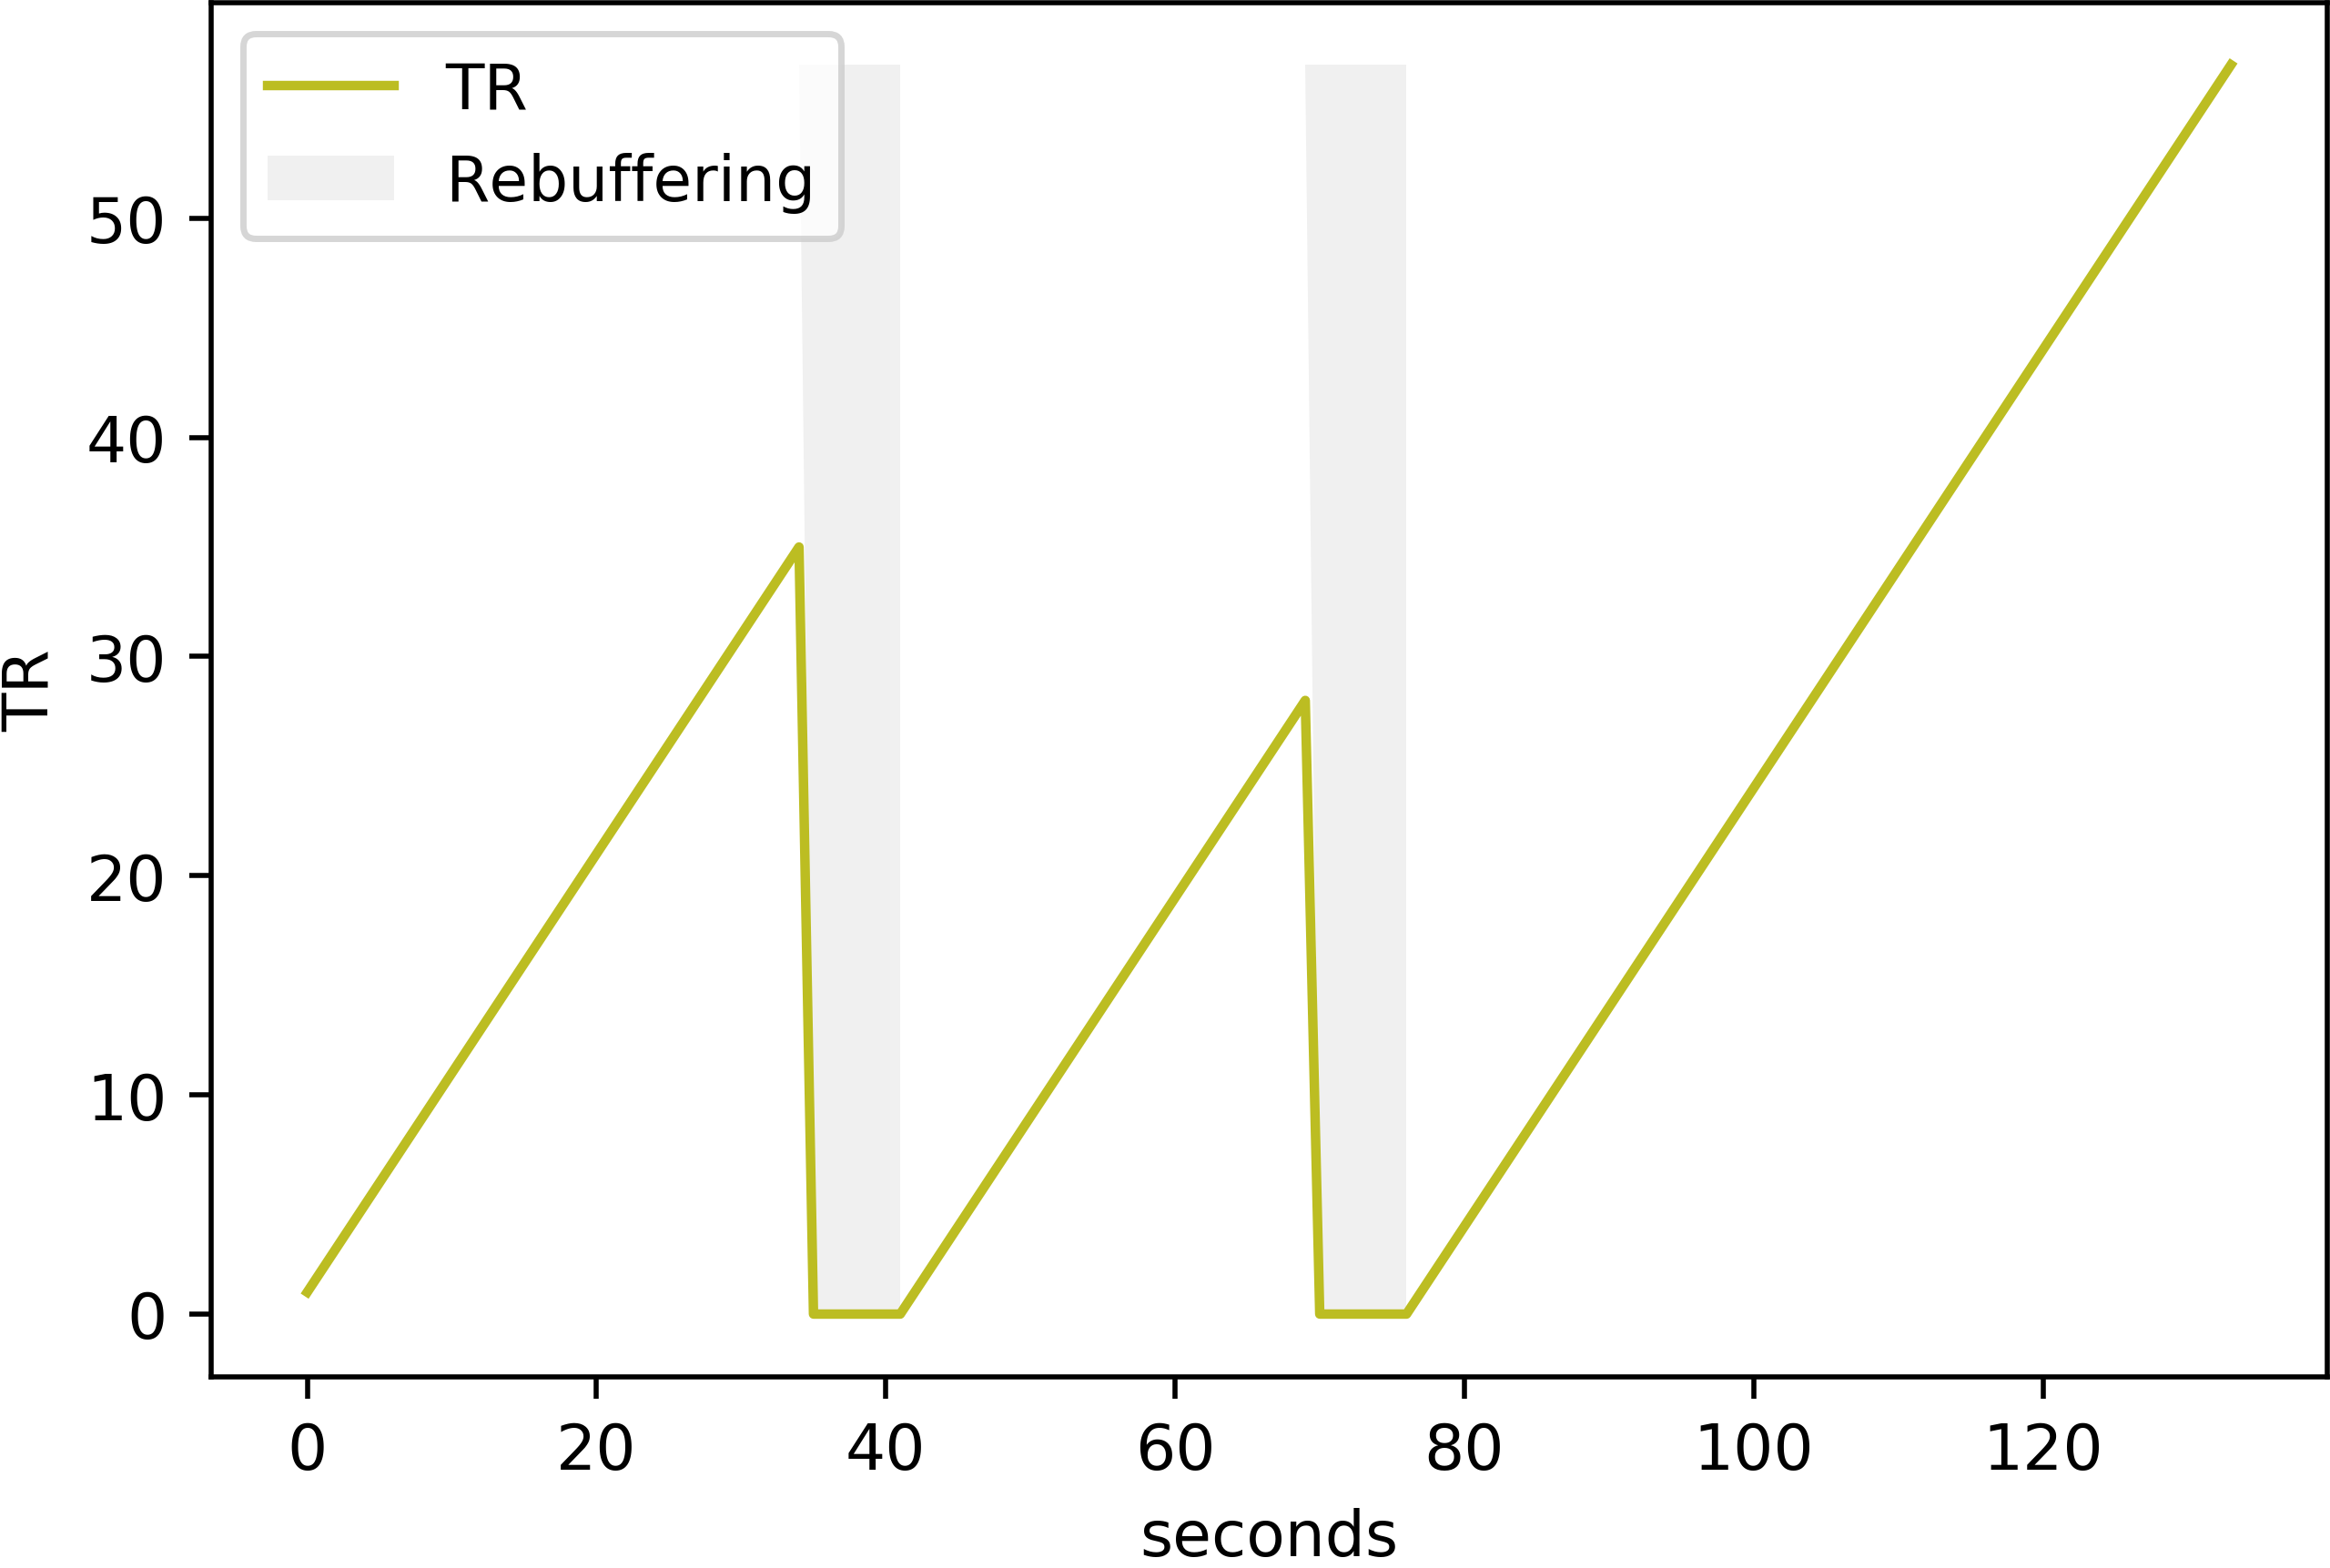
\includegraphics[width=\textwidth]{\FigsDir/features_TR.png}
    \caption{TR}
    \label{fig:InputFeatures_TR}
  \end{subfigure}
  
  \caption{Example of rebuffering and bitrate-related features represented by STSQ, PI, NR, and TR}
  \label{fig:InputFeatures}
\end{figure}


Video streaming users are sensitively affected by the video quality, known as \textit{short time subjective quality} (STSQ) \cite{QoEModel_TimeVaryingSubjectiveQuality}.
STSQ is defined as the visual quality of video being rendered to the user and can be predicted using any of the robust video quality assessment (VQA) metrics, such as Spatio-Temporal Reduced Reference Entropic Differences (STRRED) \cite{STRRED}, Multi-Scale Structural Similarity (MS-SSIM) \cite{MSSSIM}, Peak Signal to Noise Ratio (PSNR) \cite{PSNR}, etc.
Recent experiments have demonstrated that STRRED is a robust and high-performing VQA model when being tested on a very wide spectrum of video quality datasets, on multiple resolution and device types \cite{FeaturePredictionQoE, QoEModel_NLSS, QoEModel_LSTM}.
Therefore, STRRED is utilized to measure the STSQ.

Rebuffering greatly impacts the user's QoE \cite{StallingEvents}.
Thus, rebuffering information such as rebuffering length, rebuffering position and the number of rebuffering events must be investigated.
As a result, two rebuffering-related inputs are employed.
Firstly, \textit{playback indicator} (PI) \cite{QoEModel_NARX_DynamicNetworks, QoEModel_NLSS, QoEModel_LSTM} is defined as a binary continuous-time variable, specifying the current playback status, i.e., $1$ for rebuffering and $0$ for normal playback.
Secondly, as the user's annoyance increases whenever a rebuffering event occurs \cite{StallingEvents}, the \textit{number of rebuffering events} (NR) happened from the start to the current time instant of the session is considered.

Besides, the user's QoE is also affected by memory factors.
For example, more recent experiences have larger impacts on the user's perceived video quality, known as the recency effect \cite{Recency, NetflixQoE, LFOVIA}.
To capture the relation between the recency effect and the user's QoE, \textit{time elapsed since the last video impairment} (i.e., bitrate switch or rebuffering occurrence) \cite{QoEModel_NARX_DynamicNetworks, QoEModel_NLSS, QoEModel_LSTM}, denoted as TR, is utilized.


All the considered QoE influence factors are fed to the BiLSTM-QoE model to predict the instantaneous QoE. The examples of four factors (including STSQ, PI, NR, and TR) are illustrated in Figure \ref{fig:InputFeatures}.




\subsection{LIVE Netflix Video QoE Database}


The BiLSTM-QoE model is evaluated on the LIVE Netflix Video QoE Database \citep{NetflixQoE}.
The database consists of 112 distorted videos generated from 14 video contents by 8 different playout patterns
including bitrate changing, rebuffering events and mixtures of both \citep{NetflixQoE}.
The training and testing strategy are defined in \citep{QoEModel_LSTM}.
For each video $j$ in the database, one train-test set is created,
the model is trained on the set of videos that do not have the same content
and the playout pattern as the video $j$ in the test set.
Therefore, there are 112 train-test sets, each contains 1 testing videos and 91 training videos
(excludes 14 videos with the same content and 7 with the same playout pattern).
With this strategy, content and pattern dependencies are eliminated.




\subsection{Evaluation Results}


\Figure[tb][width=\linewidth]{\FigsDir/results.png}
  {QoE prediction performance of the BiLSTM-QoE over the LIVE Netflix Video QoE Database.\label{fig:BiLSTM_Accuracy}}
\Table[b]{\TablesDir/accuracy}
  {QoE prediction performance of the BiLSTM-QoE over the LIVE Netflix Video QoE Database.\label{tbl:BiLSTM_Accuracy}}


The BiLSTM-QoE model was trained and tested as described above.
The QoE prediction on the database using 4 features (i.e. STSQ, PI, TR and NR) are illustrated in Figure 6. 
The mean QoE prediction performance results are tabulated in Table \ref{tbl:BiLSTM_Accuracy},
also compared with other QoE models in the same database.
There are three considered evaluation criteria: Pearson Correlation Coefficient (PCC), Spearman Rank Correlation Coefficient (SROCC), and Root Mean Squared Error (RMSE).
The proposed model outperforms LSTM-QoE \citep{QoEModel_LSTM}, NLSS-QoE \citep{QoEModel_NLSS} and NARX \citep{QoEModel_NARX_DynamicNetworks} in terms of QoE prediction accuracy.
This is because the BiLSTM networks are very suitable to learn more useful information from time-varying features,
thereby allows this model to achieve the best performance among all the referenced models.